\section{Introduction}
% The intricate configuraton of network devices is notoriously hard to get right, forcing network 
% engineers to accept the reality of Murphy's Law or getting some help from a tool to ensure their 
% correctness, namely, network verifier.
% Over the last decade, there has been a lot of development in the area of network verification 
% generally \cite{hsa}\cite{veriflow}.
% While their approach varies a lot (e.g. data plane vs. control plane verification, deterministic vs. 
% probabilistic), most of these verifiers shares a common focus, primarily fixated on verifying 
% \textit{qualitative} properties -- the convergent functional behavior of a network under various failure 
% scenarios -- such as reachability and loop detection.

Many modern network deployments often necessitate tight performance guarantee in order to sustain 
their increasing demand.
At the same time, end users also have a rising performance standard with regards to their internet browsing 
experience, forcing companies to optimize every stack of their deployment in order to increase conversion.
Hence, network operator must find a way to verify that the network that they configure meets this demand, or 
accept the reality of Murphy's Law.

Verification of network properties related to performance metric, like bandwidth and latency, is inherently 
more challenging than a classic reachabality-based property since it introduces more dimension to the problem.
In addition to reasoning about the existence of a flow, one needs to reason about the measured 
detail of said flow and model their interaction.

Recently, there has been a few notable works that push network verification concept towards this direction 
\cite{qarc}\cite{pita}\cite{ccac}.
These \textit{quantitative} verifier model a wide range of additional network behavior that might affect 
performance to answer a specific question in mind, such as link-load violation and congestion control behavior.
However, their approaches so far has been focused on worst-case analysis, modeling and answering whether 
an unwanted event could happen or not, which requires further statistical interpretation in order to translate 
them to a percentage guarantee that appear on an SLA.

Moreover, none of these tools were designed to answer questions related to end-to-end latency, 
which is one of many important property that needs to be made certain by network providers \cite{Verizon}.
Ideally, such a tool would answer the challenge of modeling various latency altering network behavior, 
such as traffic generation, load balancing scheme, and congestion control, and expresses the important 
statistical property of the resulting end-to-end latency.
This is done not just in terms of worst-case behaviors and tails, but also the means.

In this work, we propose a verification framework to probabilistically verify the latency property of packets 
traversing from a source to destination node under various failure scenarios, by using latency 
measurements of the components in the network.

We introduce the design and implementation of \tool, a probabilistic network latency verification 
framework.
\tool will use the latency information from relevant component measurements (e.g. router queue length) 
to infer the latency distribution of said component.
Assuming that future traffic is i.i.d., we then employ a numerical convolution method to combine the
latency distribution of each relevant components together to produce the end-to-end latency distribution 
of an src-dst router pair. 

To determine said relevant components, we built \tool on top of an existing qualitative verification 
framework to efficiently explore the path used for an src-dst router pair given various scenarios of 
failures.
By obtaining the end-to-end latency distribution from this information and the latency measurement, 
we could analyze the statistical properties of the src-dst pair latency distribution to probabilistically 
argue about the latency properties.

We also introduced two optimization techniques on top of this framework to reduce the verification time 
by multiple orders of magnitude.
These two optimization techniques rely on the symmetry that we have found in the quantitative verifier 
when brought into the context of latency verification.

Our evaluation shows that the verification framework, with the help of our optimization techniques, 
could accomplish the verification task on various WAN and datacenter topologies around 90\% faster than 
our unoptimized baseline.
Moreover, highly symmetrical topology, like Fat Tree, benefits from our optimization the most 
and could reduce the verification time up to 6 orders of magnitude.

With this work, we make the following technical contributions:
\begin{itemize}
    \item \textbf{Novel temporal verification framework} using numerical convolution of network 
        components' latency measurement.
    \item \textbf{Two optimization techniques} in said verification framework by exploiting 
        symmetry in the failure exploration.
    \item \textbf{\tool}, an implementation of our verification framework and its optimization 
        on Julia.
\end{itemize}

The code for this work is open-sourced on GitHub. %TODO: change link
This work does not raise any ethical issues.

\begin{figure*}[h]
    \centering
    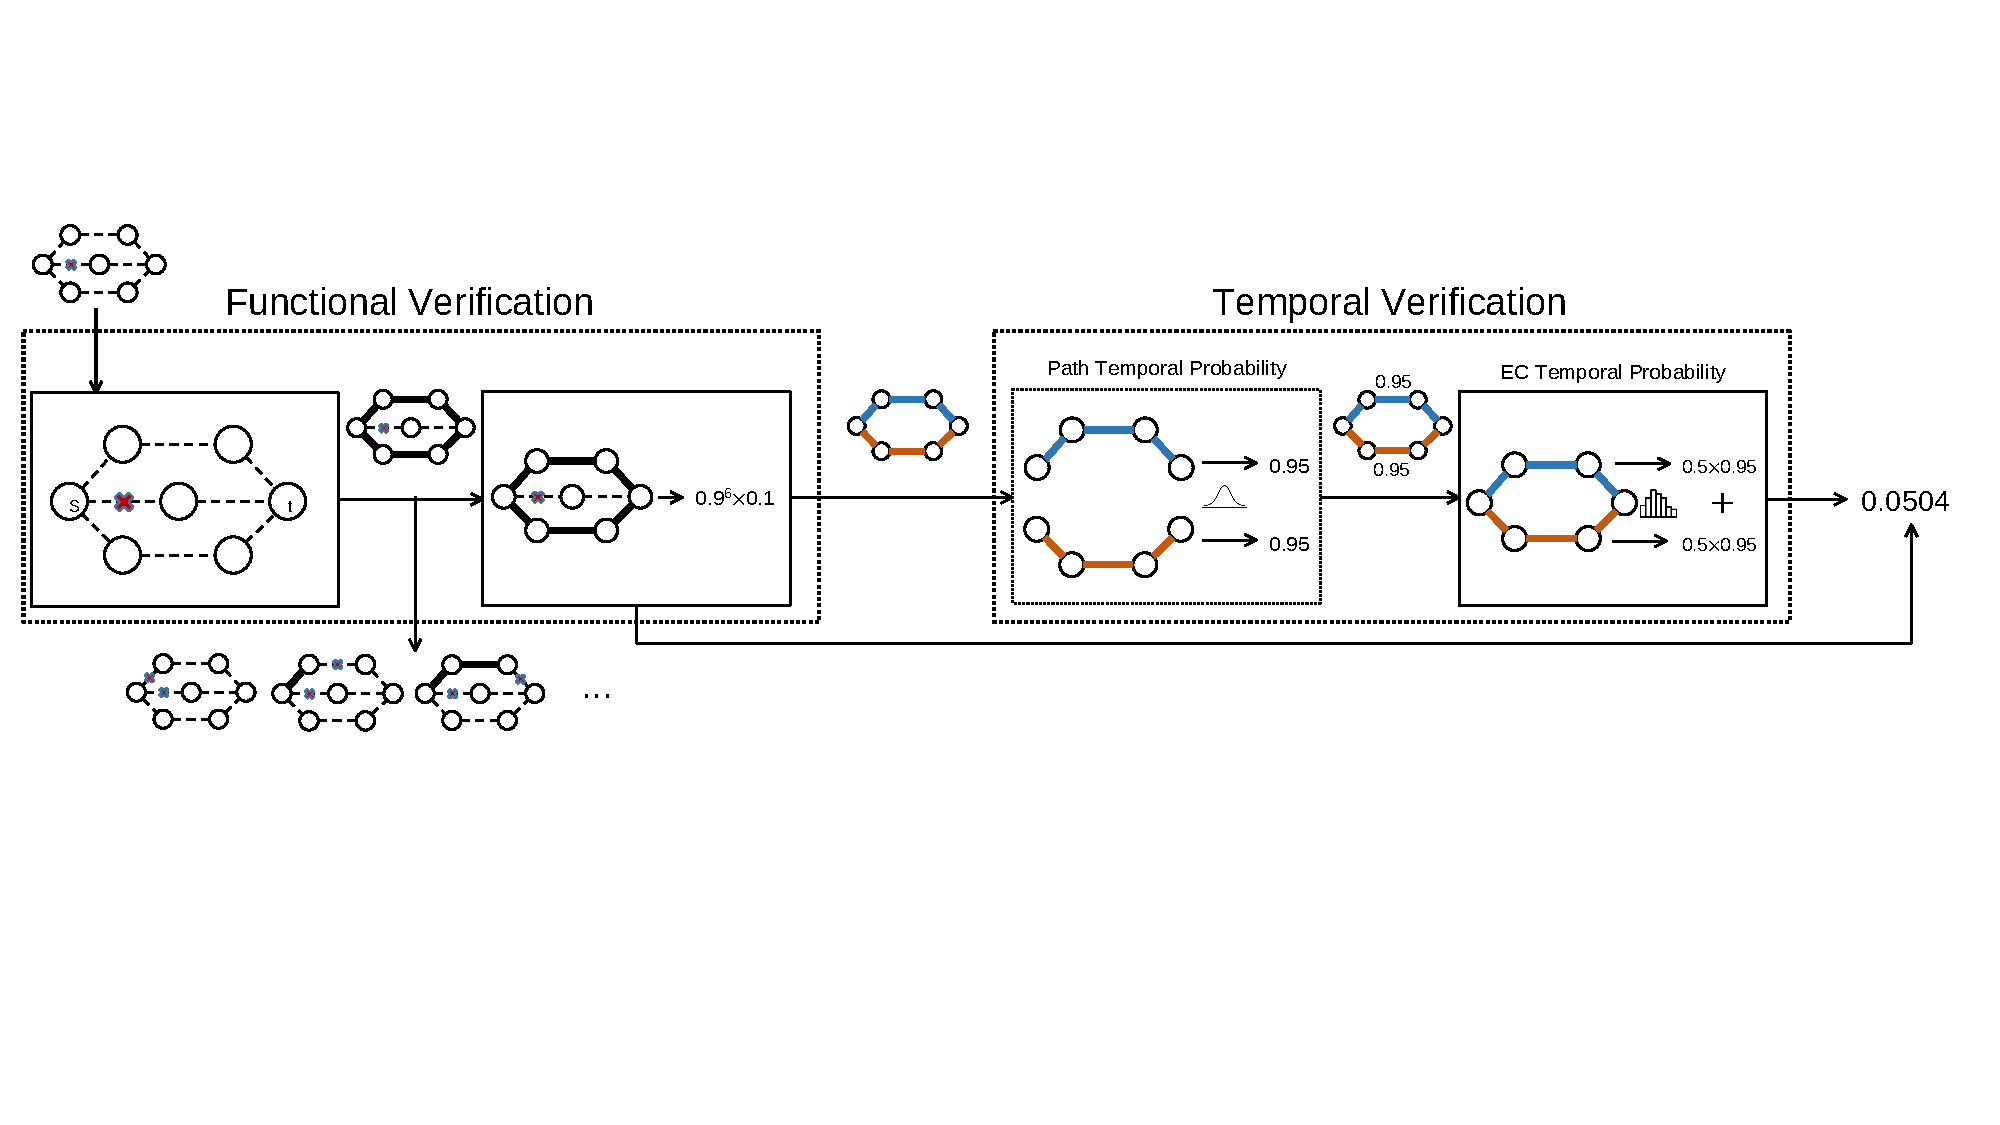
\includegraphics[scale=0.5]{overall}
    \caption{Overview of Tempus}
    \label{fig:process}
\end{figure*}